\documentclass{extbook}[14pt]
\usepackage{multicol, enumerate, enumitem, hyperref, color, soul, setspace, parskip, fancyhdr, amssymb, amsthm, amsmath, bbm, latexsym, units, mathtools}
\everymath{\displaystyle}
\usepackage[headsep=0.5cm,headheight=0cm, left=1 in,right= 1 in,top= 1 in,bottom= 1 in]{geometry}
\pagestyle{fancy}
\lhead{}
\chead{Answer Key for Module\,11L\,-\,Introduction\,to\,Limits Version A}
\rhead{}
\lfoot{Summer\,C\,2020}
\cfoot{}
\rfoot{}
\begin{document}
\textbf{This key should allow you to understand why you choose the option you did (beyond just getting a question right or wrong). \href{https://xronos.clas.ufl.edu/mac1105spring2020/courseDescriptionAndMisc/Exams/LearningFromResults}{More instructions on how to use this key can be found here}.}

\textbf{If you have a suggestion to make the keys better, \href{https://forms.gle/CZkbZmPbC9XALEE88}{please fill out the short survey here}.}

\textit{Note: This key is auto-generated and may contain issues and/or errors. The keys are reviewed after each exam to ensure grading is done accurately. If there are issues (like duplicate options), they are noted in the offline gradebook. The keys are a work-in-progress to give students as many resources to improve as possible.}

\rule{\textwidth}{0.4pt}

1. Evaluate the one-sided limit of the function $f(x)$ below, if possible.
\[ \lim_{x \rightarrow 8^-} \frac{3}{(x-8)^5}+5 \] 
The solution is $ -\infty $ 

\begin{enumerate}[label=\Alph*.] 
\item $ -\infty $ 

  
\item $ \infty $ 

  
\item $ f(8) $ 

  
\item $ \text{The limit does not exist} $ 

  
\item $ \text{None of the above} $ 

  
\end{enumerate} 
 
\textbf{General Comment:} \textbf{General comments:} You should be able to graph the rational function displayed. If not, go back to Module 7 to learn about the general shape of rational functions. 

-----------------------------------------------

2. Based on the information below, which of the following statements is always true?
$f(x)$ approaches $4.19$ as $x$ approaches $\infty$. 
The solution is $ \text{None of the above are always true.} $ 

\begin{enumerate}[label=\Alph*.] 
\item $ f(x) \text{ is close to or exactly } \infty \text{ when } x \text{ is large enough}. $ 

  
\item $ f(x) \text{ is close to or exactly } 4.19 \text{ when } x \text{ is large enough}. $ 

  
\item $ f(x) \text{ is undefined when } x \text{ is large enough}. $ 

  
\item $ f(x) \text{ is undefined when } f(x) \text{ is large enough}. $ 

  
\item $ \text{None of the above are always true.} $ 

  
\end{enumerate} 
 
\textbf{General Comment:} \textbf{General comments:} The limit tells you what happens as the $x$-values approach $\infty$. It says \textbf{absolutely nothing} about what is happening exactly at $f(x)$! 

-----------------------------------------------

3. For the graph below, evaluate the limit: $ \displaystyle \lim_{x \rightarrow -2} f(x)$.
\begin{center} 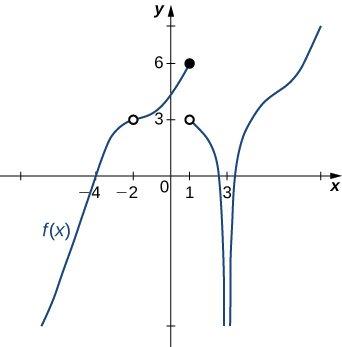
\includegraphics[width=0.3\textwidth]{../Figures/evaluateLimitGraphicallyA.png} \end{center} 

The solution is $ 3 $ 

\begin{enumerate}[label=\Alph*.] 
\item $ -\infty $ 

  
\item $ -2 $ 

  
\item $ 3 $ 

  
\item $ \text{The limit does not exist} $ 

  
\item $ \text{None of the above} $ 

  
\end{enumerate} 
 
\textbf{General Comment:} \textbf{General Comments:} Remember that the limit does not exist if the left-hand and right-hand limits do not match. 

-----------------------------------------------

4. Evaluate the limit below, if possible.
\[ \lim_{x \rightarrow 4} \frac{\sqrt{6x - 8} - 4}{7x - 28} \] 
The solution is $ \text{None of the above} $ 

\begin{enumerate}[label=\Alph*.] 
\item $ \infty $ 

 You likely believed that since the denominator is equal to 0, the limit is infinity. 
\item $ 0.018 $ 

 You likely learned L'Hospital's Rule in a previous course, but misapplied it here. 
\item $ 0.350 $ 

 You likely tried to use a shortcut to find the limit of a function that only works for when the numerator/denominator are polynomials. 
\item $ 0.125 $ 

 You likely memorized how to solve the similar homework problem and used the same formula here. 
\item $ \text{None of the above} $ 

 * This is the correct option as the limit is 0.107. 
\end{enumerate} 
 
\textbf{General Comment:} \textbf{General comments:} It is difficult to imagine the graph of this function, so you need to test values close to $x = 4$. 

-----------------------------------------------

0. To estimate the one-sided limit of the function below as $x$ approaches 1 from the left, which of the following sets of numbers should you use?
\[ \frac{\frac{1}{x} - 1}{x - 1} \] 
The solution is $ \{ 0.9000, 0.9900, 0.9990, 0.9999 \} $ 

\begin{enumerate}[label=\Alph*.] 
\item $ \{ 1.0000, 0.9000, 0.9900, 0.9990 \} $ 

 If we get $\frac{0}{0}$ or $\frac{\infty}{\infty}$, the value 1 doesn't help us estimate the limit. 
\item $ \{ 1.1000, 1.0100, 1.0010, 1.0001 \} $ 

 These values would estimate the limit of 1 on the right. 
\item $ \{ 0.9000, 0.9900, 0.9990, 0.9999 \} $ 

 This is correct! 
\item $ \{ 0.9000, 0.9900, 1.0100, 1.1000 \} $ 

 These values would estimate the limit at the point and not a one-sided limit. 
\item $ \{ 1.0000, 1.1000, 1.0100, 1.0010 \} $ 

 If we get $\frac{0}{0}$ or $\frac{\infty}{\infty}$, the value 1 doesn't help us estimate the limit. 
\end{enumerate} 
 
\textbf{General Comment:} \textbf{General Comments:} To evaluate a one-sided limit, we want to put numbers close to the limit. We can't use the limit value itself if it results in $\frac{0}{0}$ or $\frac{\infty}{\infty}$ 

-----------------------------------------------


\end{document}

